
\begin{figure}[h!]
    \centering
    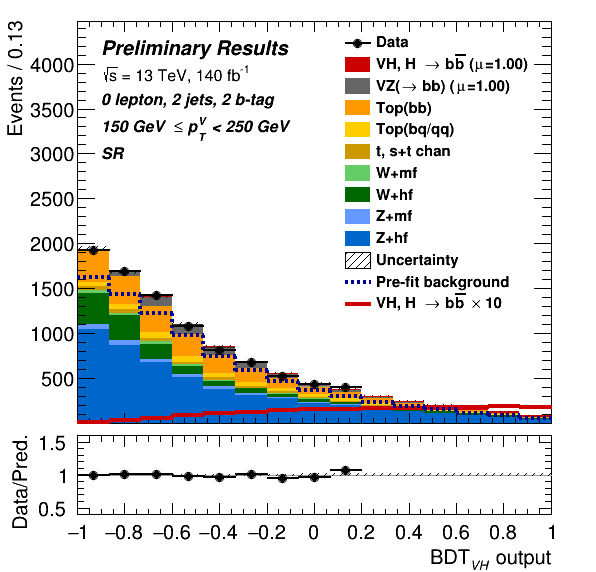
\includegraphics[width=0.32\textwidth]{Images/VH/postfit_VHbb/ZeroLep/Region_distmva_BMax250_BMin150_DSR_J2_TTypebb_T2_L0_Y6051_GlobalFit_conditionnal_mu1.pdf}
    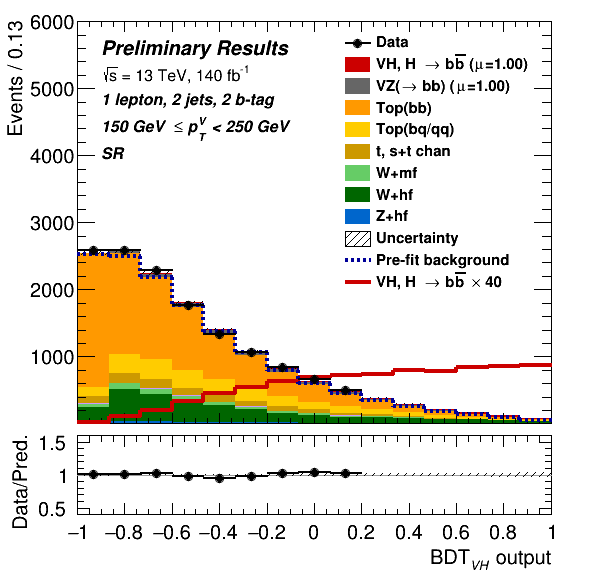
\includegraphics[width=0.32\textwidth]{ Images/VH/postfit_VHbb/OneLep/Region_distmva_BMax250_BMin150_DSR_J2_TTypebb_T2_L1_Y6051_GlobalFit_conditionnal_mu1.pdf}
    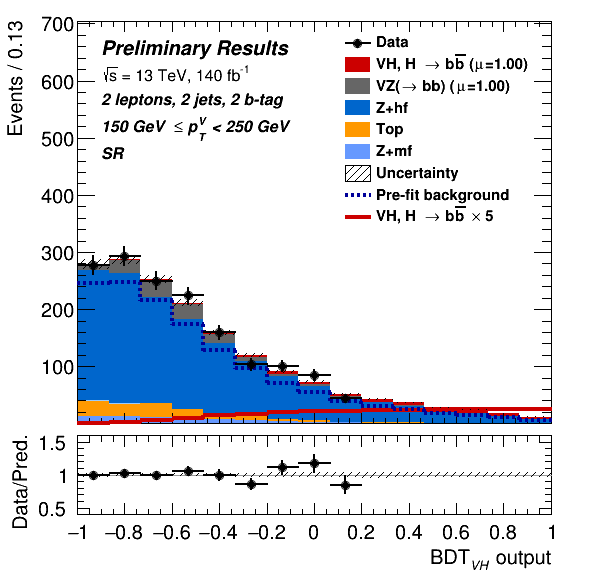
\includegraphics[width=0.32\textwidth]{ Images/VH/postfit_VHbb/TwoLep/Region_distmva_BMax250_BMin150_DSR_J2_TTypebb_T2_L2_Y6051_GlobalFit_conditionnal_mu1.pdf}
    \caption{The \vhb\ posfit conditional distribution in the 150 < \ptv\ < 250 GeV 2-jet signal region in the 0L (left), 1L (centre), and 2L (right).}
    \label{fig:plotsVHBSR_150pt_2J}
  \end{figure} 
  
  \begin{figure}[h!]
    \centering
    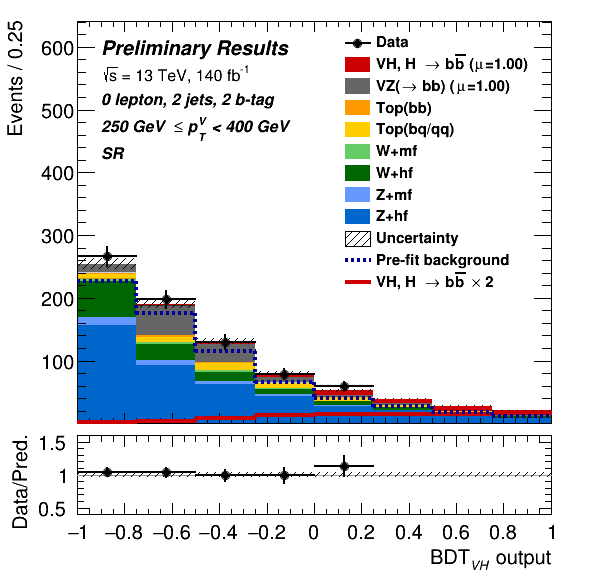
\includegraphics[width=0.32\textwidth]{Images/VH/postfit_VHbb/ZeroLep/Region_distmva_BMax400_BMin250_DSR_J2_TTypebb_T2_L0_Y6051_GlobalFit_conditionnal_mu1.pdf}
    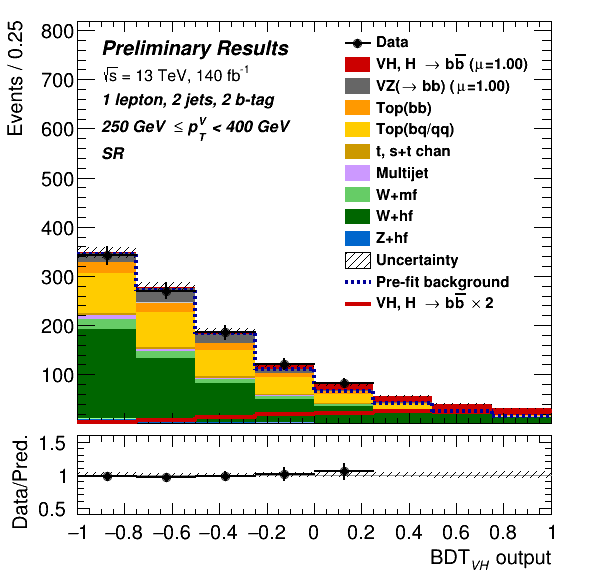
\includegraphics[width=0.32\textwidth]{ Images/VH/postfit_VHbb/OneLep/Region_distmva_BMax400_BMin250_DSR_J2_TTypebb_T2_L1_Y6051_GlobalFit_conditionnal_mu1.pdf}
    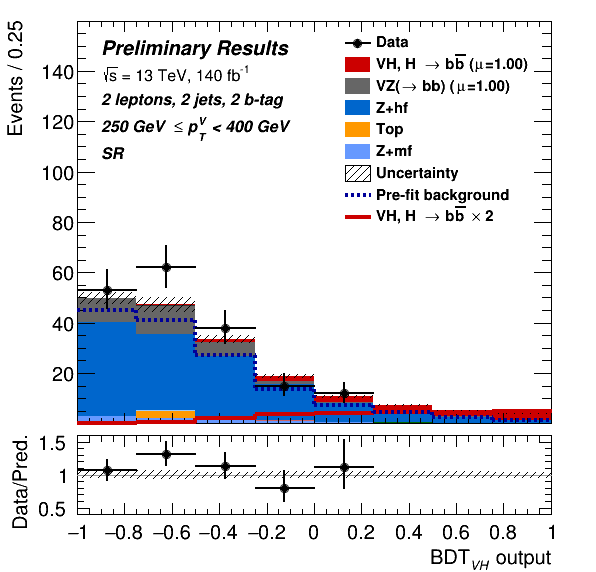
\includegraphics[width=0.32\textwidth]{ Images/VH/postfit_VHbb/TwoLep/Region_distmva_BMax400_BMin250_DSR_J2_TTypebb_T2_L2_Y6051_GlobalFit_conditionnal_mu1.pdf}
    \caption{The \vhb\ posfit conditional distribution in the 250 < \ptv\ < 400 GeV 2-jet signal region in the 0L (left), 1L (centre), and 2L (right).}
    \label{fig:plotsVHBSR_250pt_2J}
  \end{figure}
  
  \begin{figure}[h!]
    \centering
    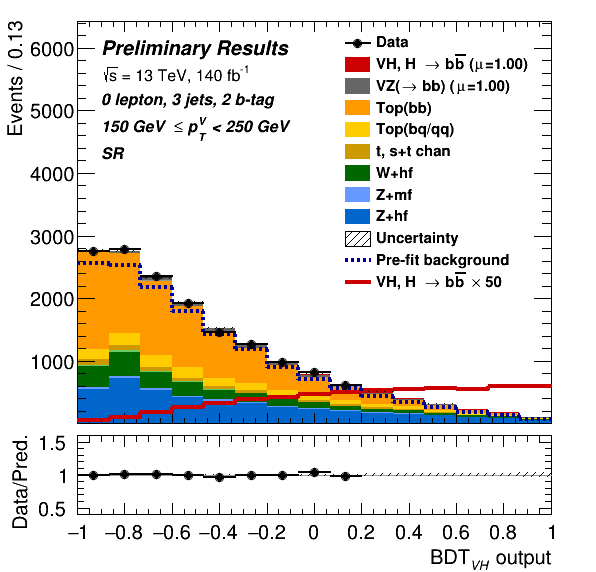
\includegraphics[width=0.32\textwidth]{Images/VH/postfit_VHbb/ZeroLep/Region_distmva_BMax250_BMin150_DSR_J3_TTypebb_T2_L0_Y6051_GlobalFit_conditionnal_mu1.pdf}
    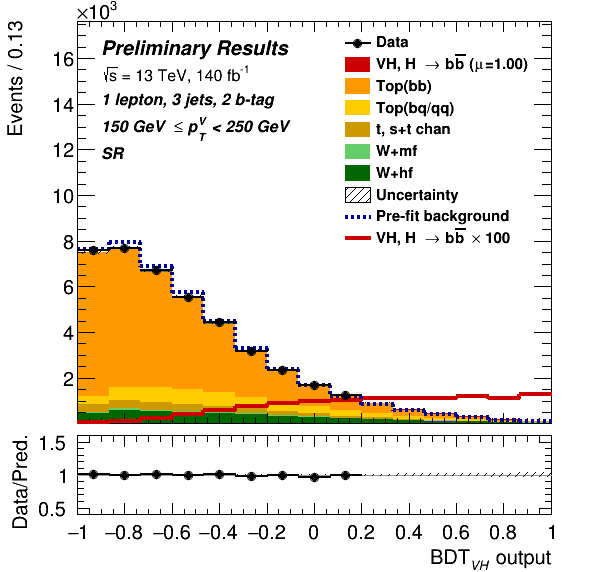
\includegraphics[width=0.32\textwidth]{Images/VH/postfit_VHbb/OneLep/Region_distmva_BMax250_BMin150_DSR_J3_TTypebb_T2_L1_Y6051_GlobalFit_conditionnal_mu1.pdf}
    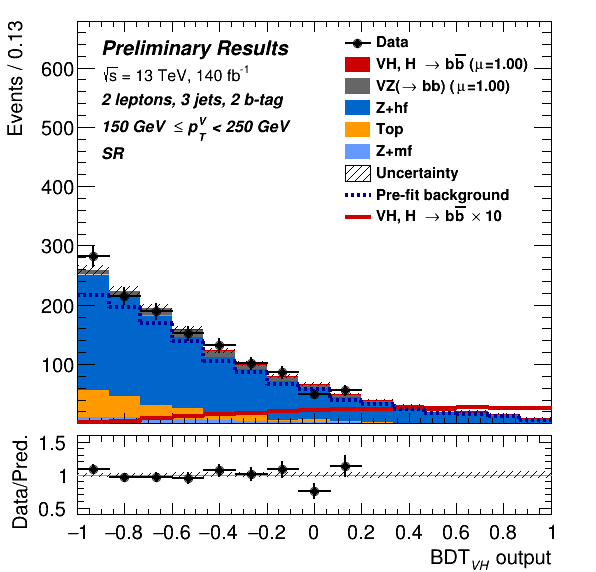
\includegraphics[width=0.32\textwidth]{Images/VH/postfit_VHbb/TwoLep/Region_distmva_BMax250_BMin150_DSR_J3_TTypebb_T2_L2_Y6051_GlobalFit_conditionnal_mu1.pdf}
    \caption{The \vhb\ posfit conditional distribution in the 150 < \ptv\ < 250 GeV 3-jet signal region in the 0L (left), 1L (centre), and 2L (right).}
    \label{fig:plotsVHBSR_150pt_3J}
  \end{figure} 
  
  \begin{figure}[h!]
    \centering
    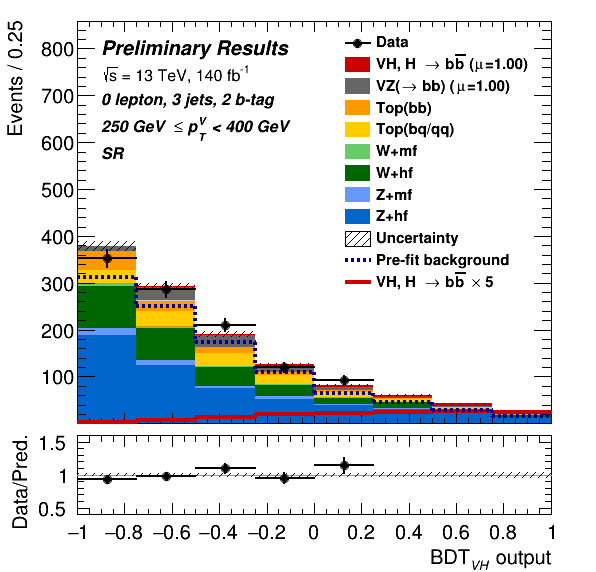
\includegraphics[width=0.32\textwidth]{Images/VH/postfit_VHbb/ZeroLep/Region_distmva_BMax400_BMin250_DSR_J3_TTypebb_T2_L0_Y6051_GlobalFit_conditionnal_mu1.pdf}
    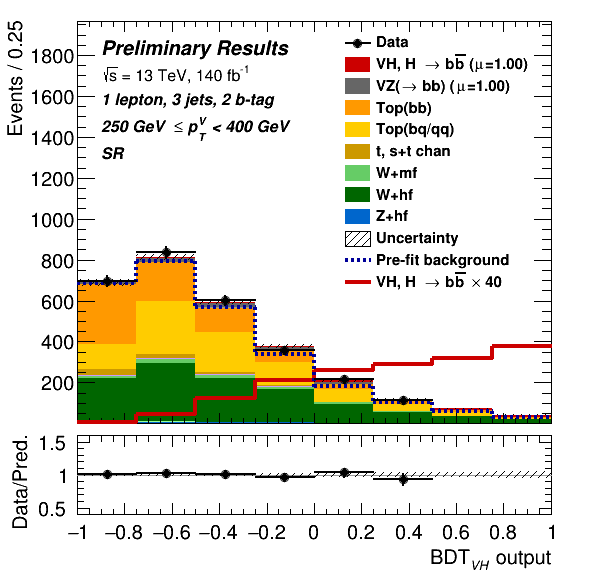
\includegraphics[width=0.32\textwidth]{ Images/VH/postfit_VHbb/OneLep/Region_distmva_BMax400_BMin250_DSR_J3_TTypebb_T2_L1_Y6051_GlobalFit_conditionnal_mu1.pdf}
    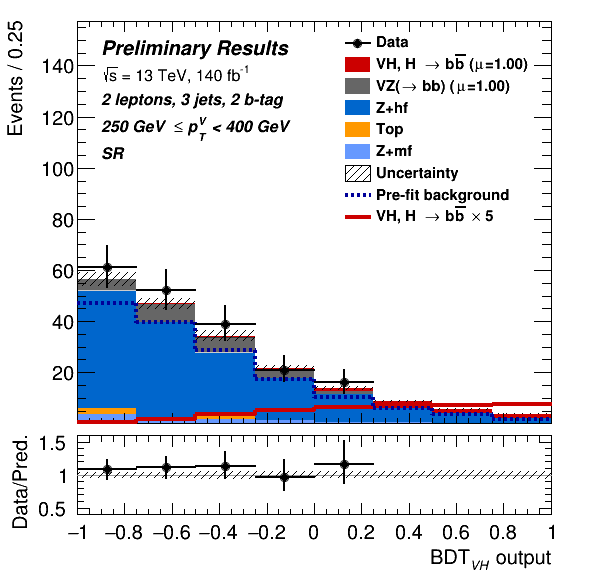
\includegraphics[width=0.32\textwidth]{ Images/VH/postfit_VHbb/TwoLep/Region_distmva_BMax400_BMin250_DSR_J3_TTypebb_T2_L2_Y6051_GlobalFit_conditionnal_mu1.pdf}
    \caption{The \vhb\ posfit conditional distribution in the 250 < \ptv\ < 400 GeV 3-jet signal region in the 0L (left), 1L (centre), and 2L (right).}
    \label{fig:plotsVHBSR_250pt_3J}
  \end{figure} 
  
  % 4J mid pTV
  \begin{figure}[h!]
    \centering
    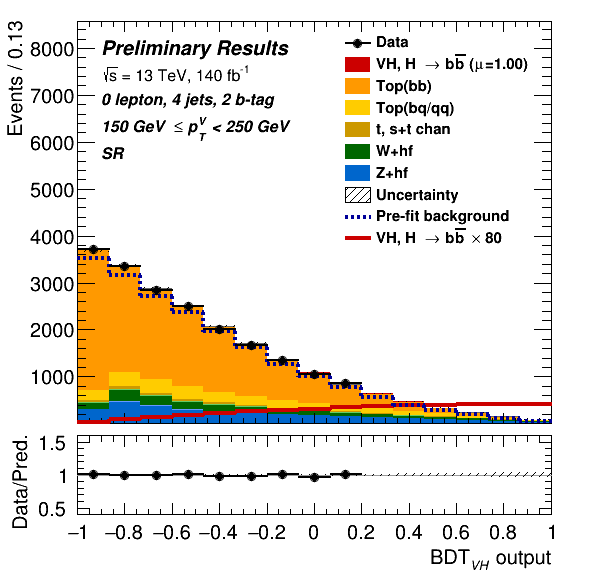
\includegraphics[width=0.24\textwidth]{Images/VH/postfit_VHbb/ZeroLep/Region_distmva_BMax250_BMin150_DSR_J4_TTypebb_T2_L0_Y6051_GlobalFit_conditionnal_mu1.pdf}
    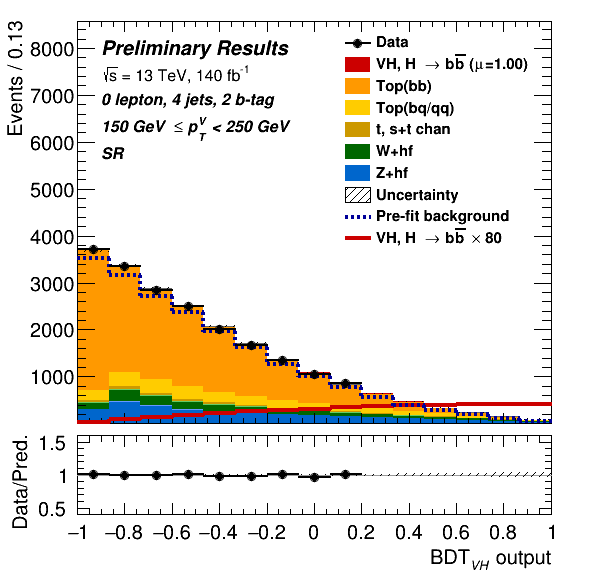
\includegraphics[width=0.24\textwidth]{Images/VH/postfit_VHbb/ZeroLep/Region_distmva_BMax250_BMin150_DSR_J4_TTypebb_T2_L0_Y6051_GlobalFit_conditionnal_mu1.pdf}
    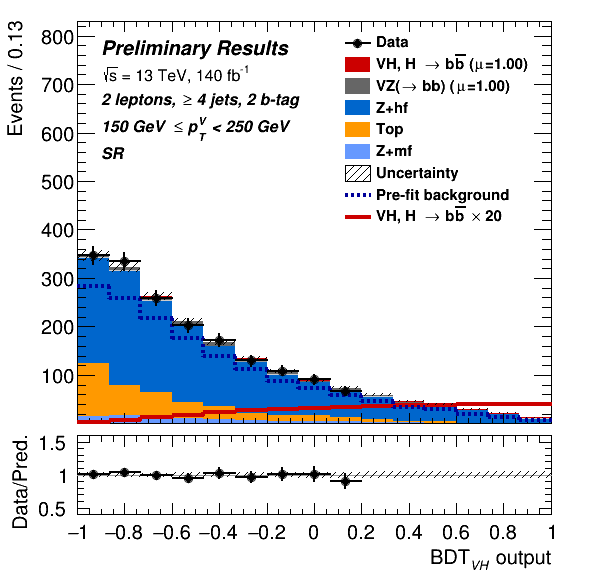
\includegraphics[width=0.24\textwidth]{ Images/VH/postfit_VHbb/TwoLep/Region_distmva_BMax250_BMin150_DSR_J4_TTypebb_incJet1_T2_L2_Y6051_GlobalFit_conditionnal_mu1.pdf}
    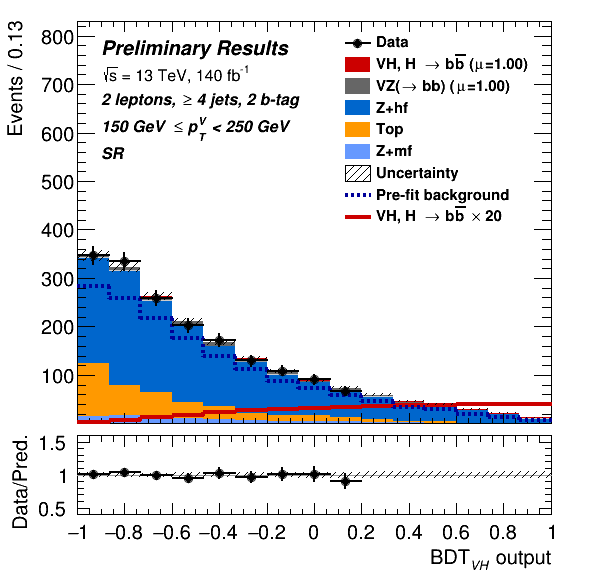
\includegraphics[width=0.24\textwidth]{ Images/VH/postfit_VHbb/TwoLep/Region_distmva_BMax250_BMin150_DSR_J4_TTypebb_incJet1_T2_L2_Y6051_GlobalFit_conditionnal_mu1.pdf}
    \caption{The \vhb\ posfit conditional distribution in the 150 < \ptv\ < 250 GeV 4-jet (4p-jet) signal region in the 0L (2 left) and 2L (2 right).}
    \label{fig:plotsVHBSR_150pt_4J}
  \end{figure} 
  
  \begin{figure}[h!]
    \centering
    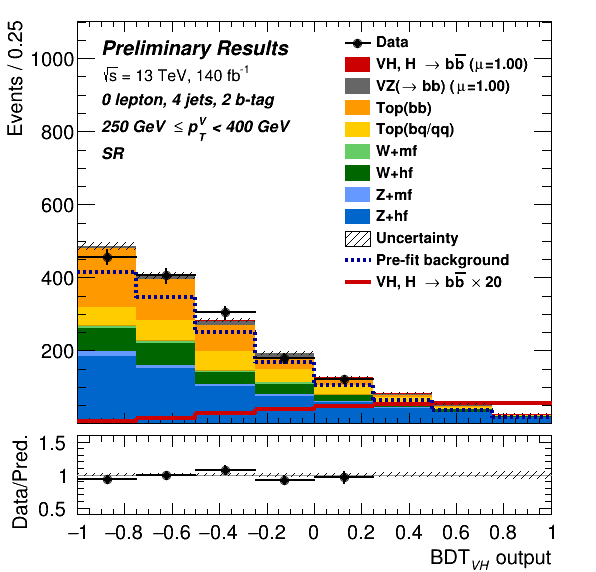
\includegraphics[width=0.24\textwidth]{Images/VH/postfit_VHbb/ZeroLep/Region_distmva_BMax400_BMin250_DSR_J4_TTypebb_T2_L0_Y6051_GlobalFit_conditionnal_mu1.pdf}
    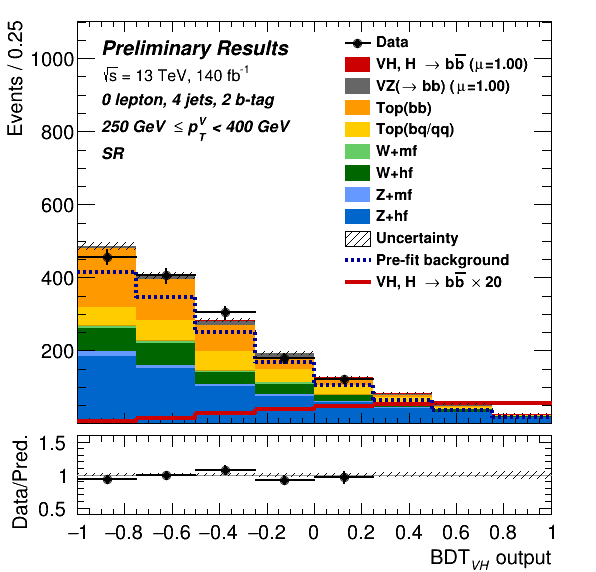
\includegraphics[width=0.24\textwidth]{Images/VH/postfit_VHbb/ZeroLep/Region_distmva_BMax400_BMin250_DSR_J4_TTypebb_T2_L0_Y6051_GlobalFit_conditionnal_mu1.pdf}
    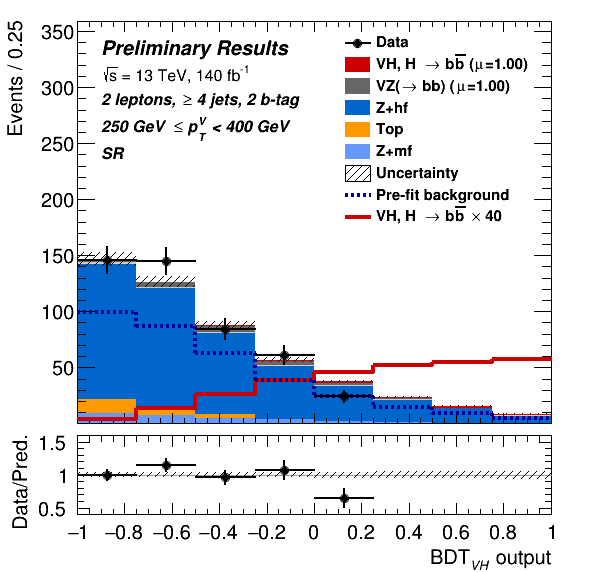
\includegraphics[width=0.24\textwidth]{ Images/VH/postfit_VHbb/TwoLep/Region_distmva_BMax400_BMin250_DSR_J4_TTypebb_incJet1_T2_L2_Y6051_GlobalFit_conditionnal_mu1.pdf}
    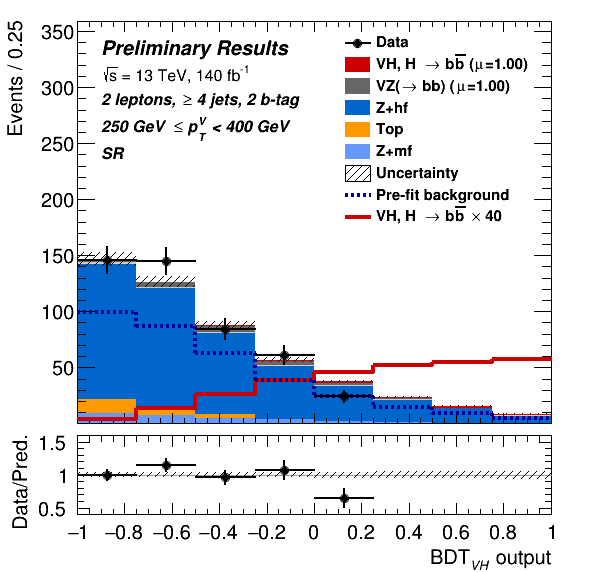
\includegraphics[width=0.24\textwidth]{ Images/VH/postfit_VHbb/TwoLep/Region_distmva_BMax400_BMin250_DSR_J4_TTypebb_incJet1_T2_L2_Y6051_GlobalFit_conditionnal_mu1.pdf}
    \caption{The \vhb\ posfit conditional distribution in the 150 < \ptv\ < 250 GeV 4-jet (4p-jet) signal region in the 0L (2 left) and 2L (2 right).}
    \label{fig:plotsVHBSR_250pt_4J}
  \end{figure} 
  
  % low pTV VHbb
  \begin{figure}[h!]
    \centering
    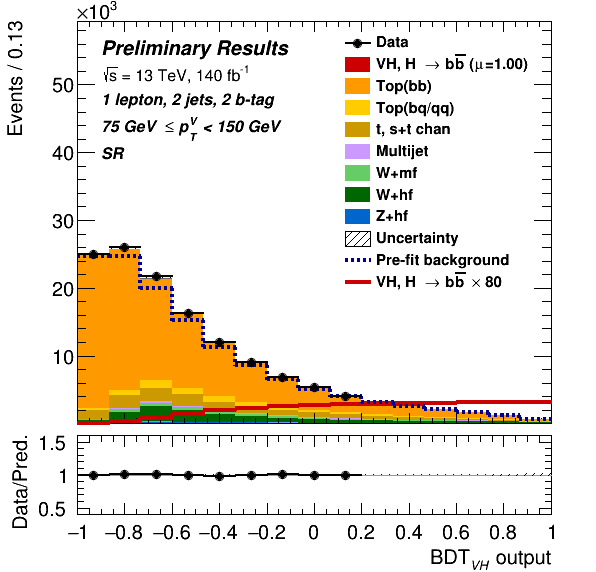
\includegraphics[width=0.32\textwidth]{Images/VH/postfit_VHbb/OneLep/Region_distmva_BMax150_BMin75_DSR_J2_TTypebb_T2_L1_Y6051_GlobalFit_conditionnal_mu1.pdf}
    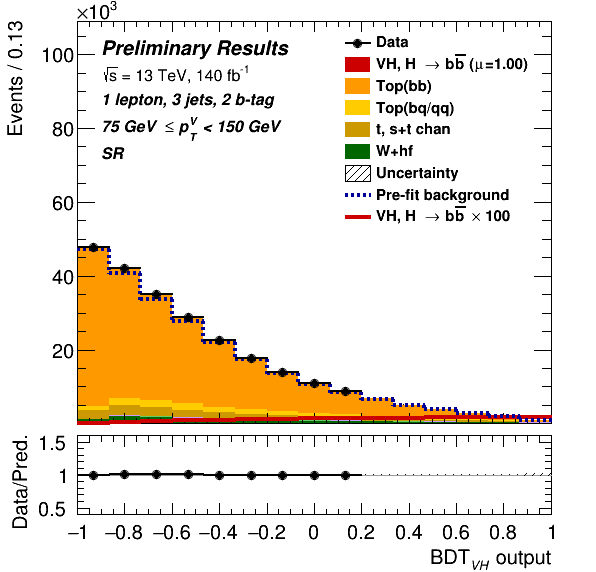
\includegraphics[width=0.32\textwidth]{Images/VH/postfit_VHbb/OneLep/Region_distmva_BMax150_BMin75_DSR_J3_TTypebb_T2_L1_Y6051_GlobalFit_conditionnal_mu1.pdf}
    \caption{The 1L \vhb\ posfit conditional distribution in the 75 < \ptv\ < 150 GeV 2-jet (left) and 3-jet (right) signal regions.}
    \label{fig:plotsVHBSR_75pt_1L}
  \end{figure} 
  
  \begin{figure}[h!]
    \centering
    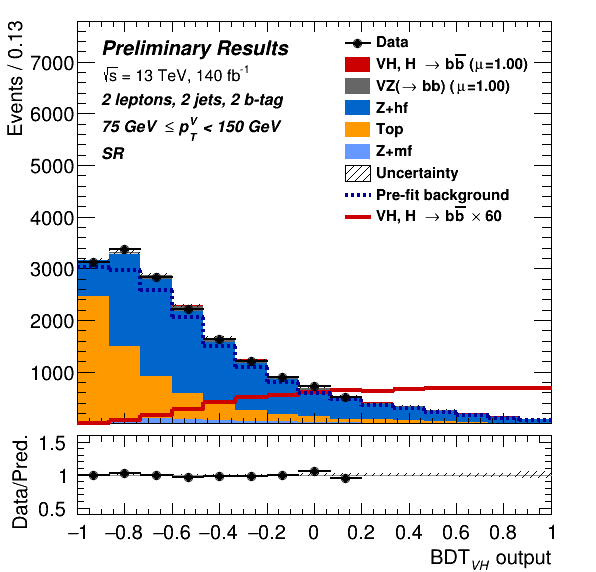
\includegraphics[width=0.32\textwidth]{Images/VH/postfit_VHbb/TwoLep/Region_distmva_BMax150_BMin75_DSR_J2_TTypebb_T2_L2_Y6051_GlobalFit_conditionnal_mu1.pdf}
    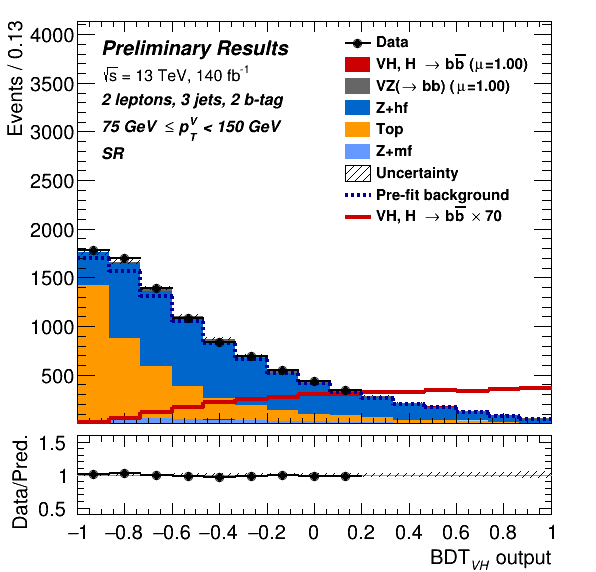
\includegraphics[width=0.32\textwidth]{Images/VH/postfit_VHbb/TwoLep/Region_distmva_BMax150_BMin75_DSR_J3_TTypebb_T2_L2_Y6051_GlobalFit_conditionnal_mu1.pdf}
    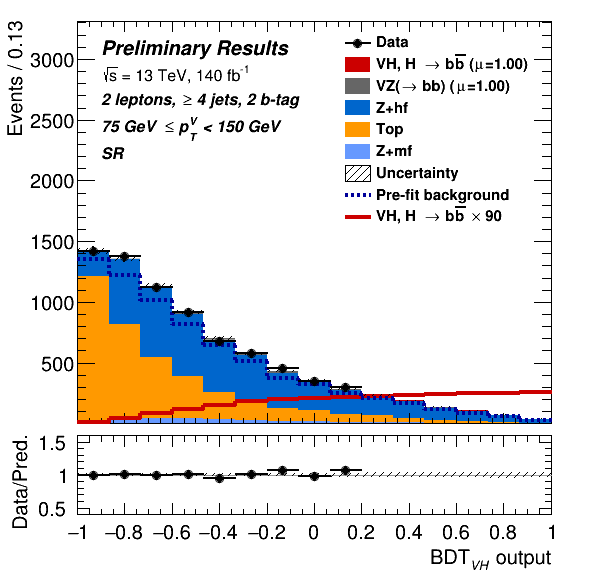
\includegraphics[width=0.32\textwidth]{Images/VH/postfit_VHbb/TwoLep/Region_distmva_BMax150_BMin75_DSR_J4_TTypebb_incJet1_T2_L2_Y6051_GlobalFit_conditionnal_mu1.pdf}
    \caption{The 2L \vhb\ posfit conditional distribution in the 75 < \ptv\ < 150 GeV 2-jet (left), 3-jet (centre) and 4p-jet (right) signal regions.}
    \label{fig:plotsVHBSR_75pt_2L}
  \end{figure} 
  
  %\begin{figure}[h!]
  %  \includegraphics[width=0.32\textwidth]{Images/VH/postfit_VHbb/ZeroLep/}
  %  \includegraphics[width=0.32\textwidth]{Images/VH/postfit_VHbb/OneLep/}
  %  \includegraphics[width=0.32\textwidth]{Images/VH/postfit_VHbb/TwoLep/}
  %  \caption{}
  %  \label{fig:plots}
  %\end{figure} 


 % ---


\begin{figure}[h!]
    \centering
    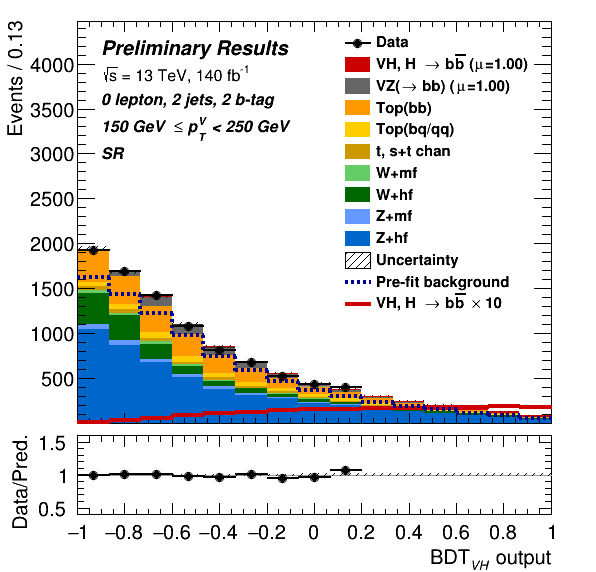
\includegraphics[width=0.32\textwidth]{Images/VH/postfit_VHbb/ZeroLep/Region_distmva_BMax250_BMin150_DSR_J2_TTypebb_T2_L0_Y6051_GlobalFit_conditionnal_mu1.pdf}
    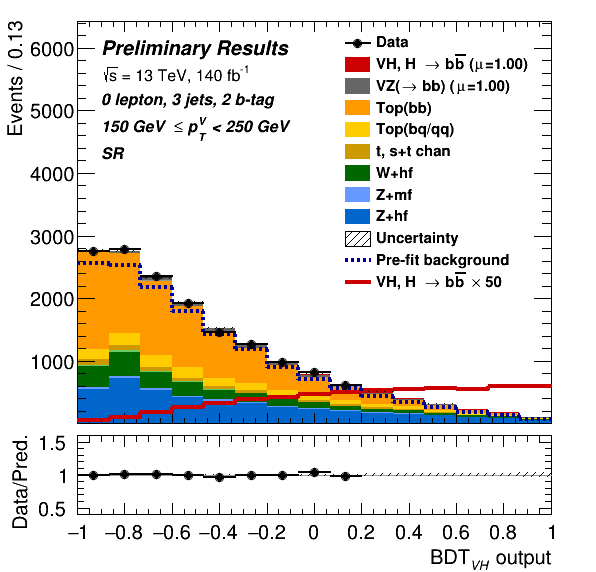
\includegraphics[width=0.32\textwidth]{Images/VH/postfit_VHbb/ZeroLep/Region_distmva_BMax250_BMin150_DSR_J3_TTypebb_T2_L0_Y6051_GlobalFit_conditionnal_mu1.pdf}
    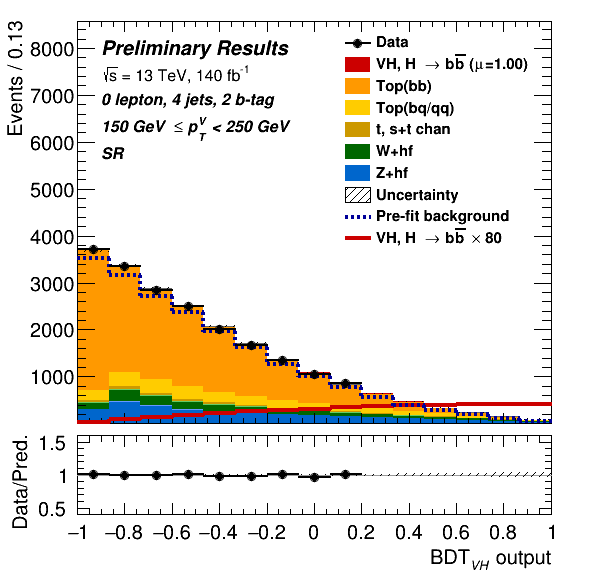
\includegraphics[width=0.32\textwidth]{Images/VH/postfit_VHbb/ZeroLep/Region_distmva_BMax250_BMin150_DSR_J4_TTypebb_T2_L0_Y6051_GlobalFit_conditionnal_mu1.pdf}
    \caption{The 0L posfit conditional distribution in the $BB$-tag, 150 < \ptv\ < 250 GeV, 2-jet(left), 3-jet (centre), and 4-jet (right) signal regions.}
    \label{fig:plotsVHBSR_150pt_0L}
\end{figure} 

\begin{figure}[h!]
    \centering
    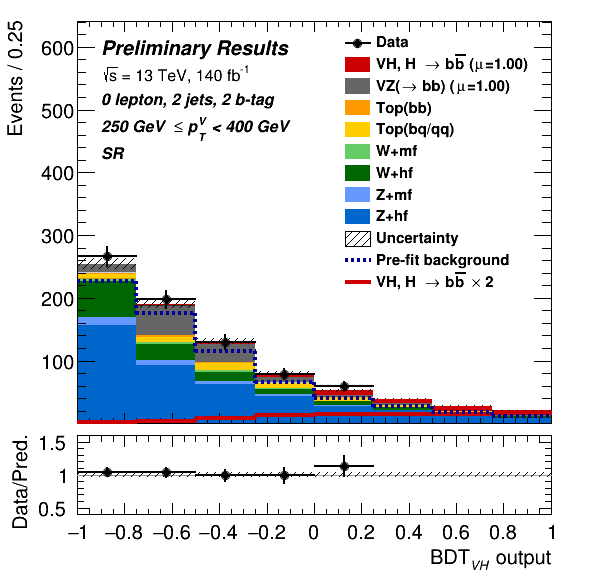
\includegraphics[width=0.32\textwidth]{Images/VH/postfit_VHbb/ZeroLep/Region_distmva_BMax400_BMin250_DSR_J2_TTypebb_T2_L0_Y6051_GlobalFit_conditionnal_mu1.pdf}
    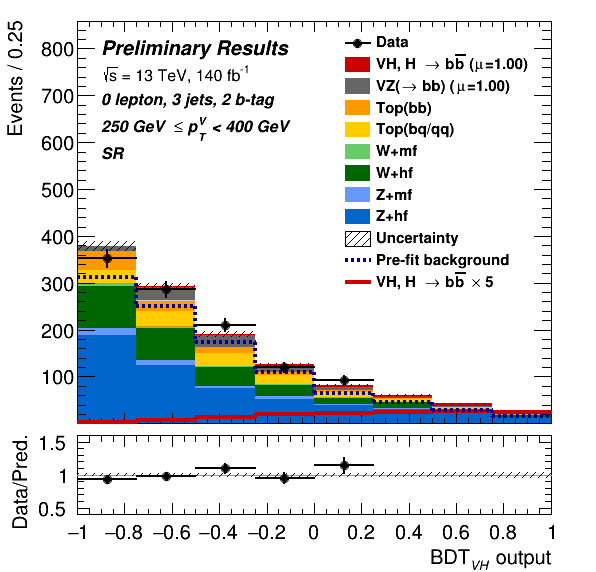
\includegraphics[width=0.32\textwidth]{Images/VH/postfit_VHbb/ZeroLep/Region_distmva_BMax400_BMin250_DSR_J3_TTypebb_T2_L0_Y6051_GlobalFit_conditionnal_mu1.pdf}
    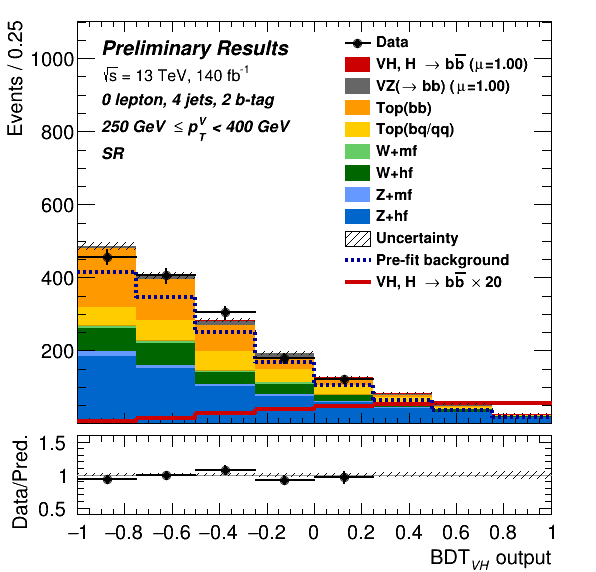
\includegraphics[width=0.32\textwidth]{Images/VH/postfit_VHbb/ZeroLep/Region_distmva_BMax400_BMin250_DSR_J4_TTypebb_T2_L0_Y6051_GlobalFit_conditionnal_mu1.pdf}
    \caption{The 0L posfit conditional distribution in the $BB$-tag, 250 < \ptv\ < 400 GeV, 2-jet(left), 3-jet (centre), and 4-jet (right) signal regions.}
    \label{fig:plotsVHBSR_250pt_0L}
\end{figure} 

\begin{figure}[h!]
    \centering
    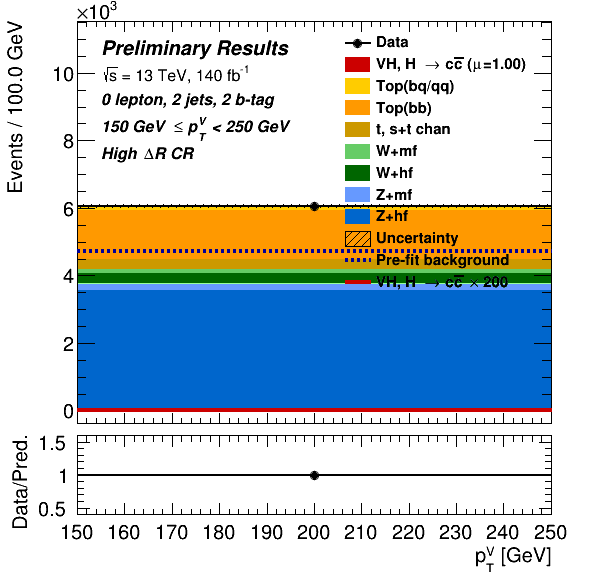
\includegraphics[width=0.32\textwidth]{Images/VH/postfit_VHbb/ZeroLep/Region_distpTV_BMax250_BMin150_DCRHigh_J2_TTypebb_T2_L0_Y6051_GlobalFit_conditionnal_mu1.pdf}
    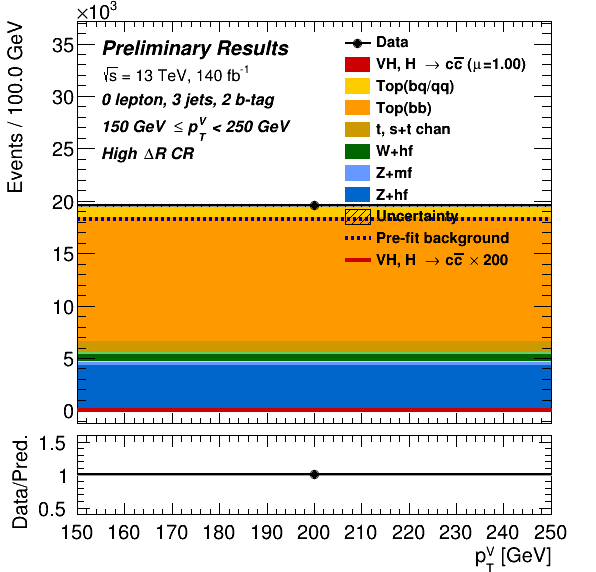
\includegraphics[width=0.32\textwidth]{Images/VH/postfit_VHbb/ZeroLep/Region_distpTV_BMax250_BMin150_DCRHigh_J3_TTypebb_T2_L0_Y6051_GlobalFit_conditionnal_mu1.pdf}
    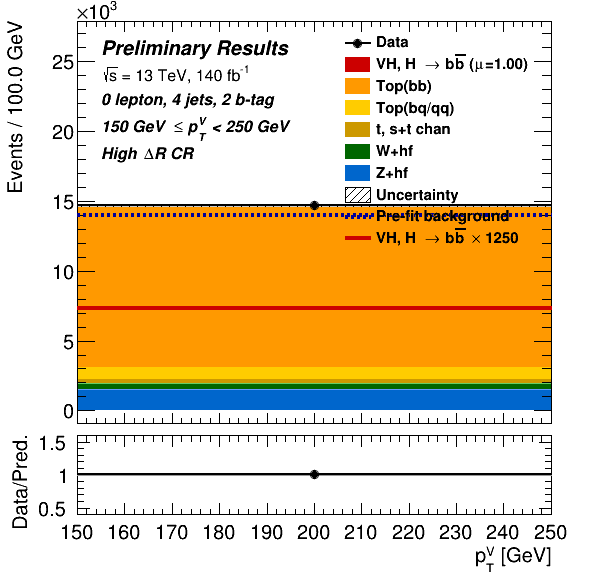
\includegraphics[width=0.32\textwidth]{Images/VH/postfit_VHbb/ZeroLep/Region_distpTV_BMax250_BMin150_DCRHigh_J4_TTypebb_T2_L0_Y6051_GlobalFit_conditionnal_mu1.pdf}
    \caption{The 0L posfit conditional distribution in the $BB$-tag, 150 < \ptv\ < 250 GeV 2-jet(left), 3-jet (centre), and 4-jet (right) signal regions.}
    \label{fig:plotsVHBSR_150pt_0L}
\end{figure} 


Region_distpTV_BMax250_BMin150_DCRHigh_J2_TTypebb_T2_L0_Y6051_GlobalFit_conditionnal_mu1.pdf
Region_distpTV_BMax250_BMin150_DCRHigh_J3_TTypebb_T2_L0_Y6051_GlobalFit_conditionnal_mu1.pdf
Region_distpTV_BMax250_BMin150_DCRHigh_J4_TTypebb_T2_L0_Y6051_GlobalFit_conditionnal_mu1.pdf

Region_distpTV_BMax400_BMin250_DCRHigh_J2_TTypebb_T2_L0_Y6051_GlobalFit_conditionnal_mu1.pdf
Region_distpTV_BMax400_BMin250_DCRHigh_J3_TTypebb_T2_L0_Y6051_GlobalFit_conditionnal_mu1.pdf
Region_distpTV_BMax400_BMin250_DCRHigh_J4_TTypebb_T2_L0_Y6051_GlobalFit_conditionnal_mu1.pdf